

In an early stage of the project, we noticed that the environment exhibits multiple spatial symmetries and though about how this can be exploited, when training an agent. Loosely speaking, if an agent knows how to act in a particular state $s$, this information can be used by the agent to act in the seven different states, which arise as symmetric transformations - flips / rotations / transposition - of the state $s$, given that its actions are transformed accordingly.
% TODO: http://www.cs.cmu.edu/~maz/publications/symmetry7.pdf
% TODO: https://alexandria.physik3.uni-goettingen.de/PDF/agostinicelaya2009
A search in relevant literature revealed that \ref{} identifies these symmetries as symmetries with \emph{adherence to an equivalence relation}. Moreover, \ref{} describes two multiple possibilities to exploit these symmetries in the training process of an agent.

\vspace{10pt}
\begin{center}
\begin{minipage}{\linewidth}
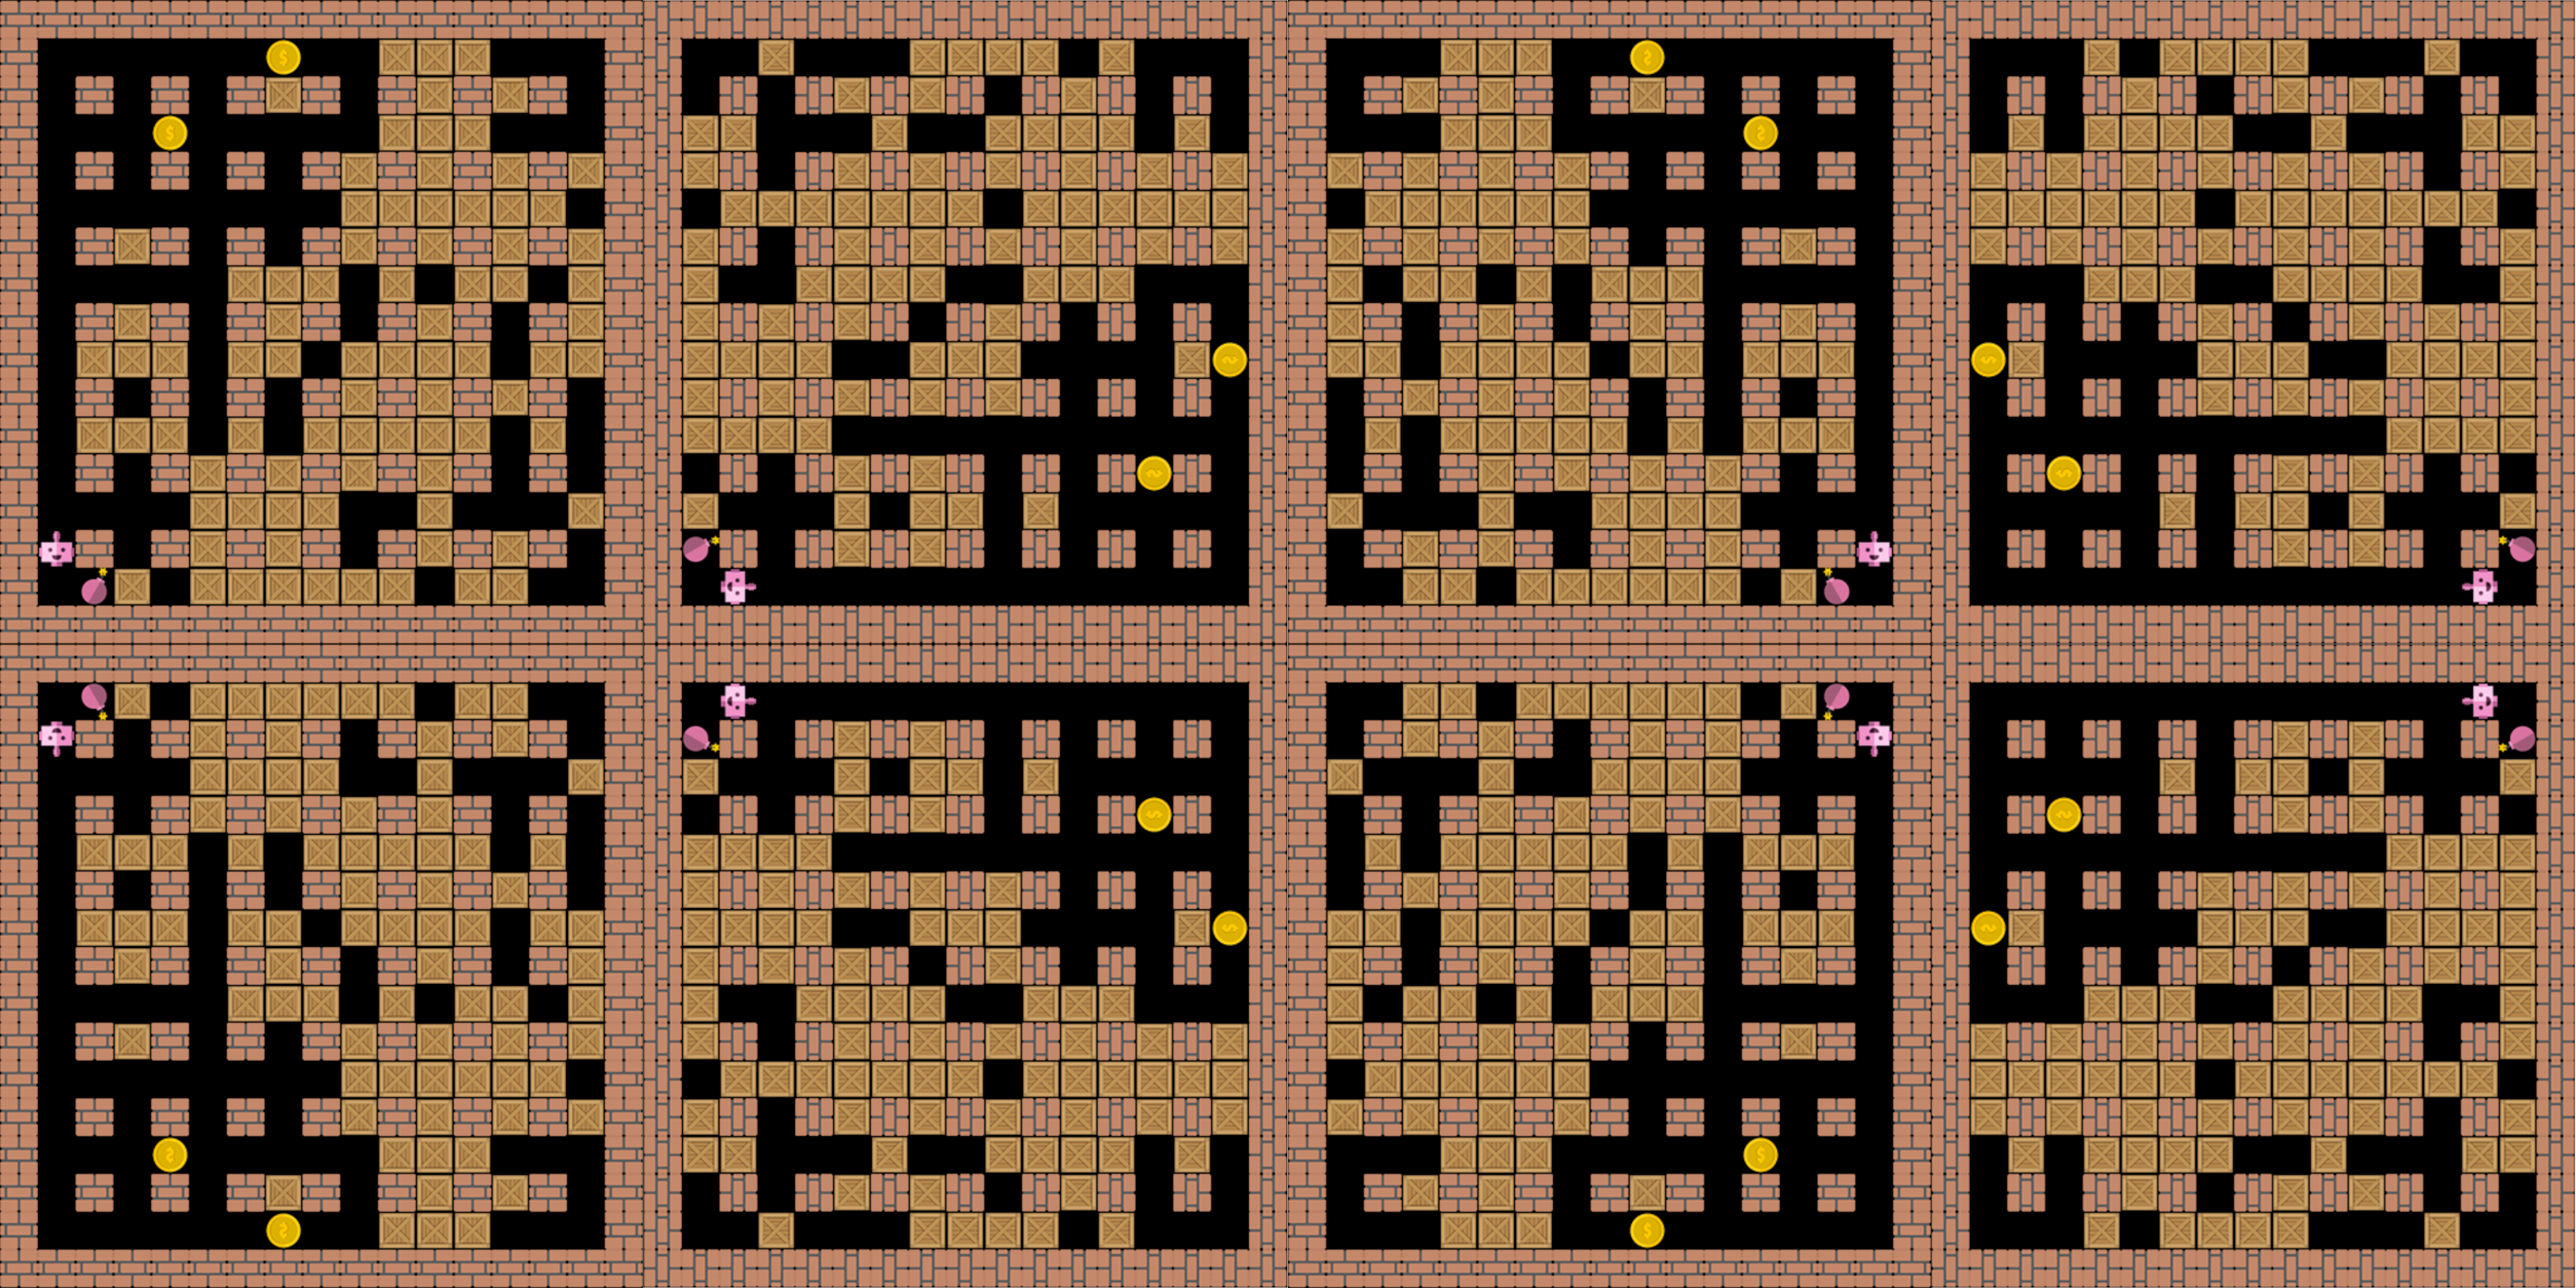
\includegraphics[scale=0.2]{graphics/symmetries.png}
\captionof{figure}{Visualisation of 8 states in the same equivalence class w.r.t. $\sim_{\text{sym}}$.}
\end{minipage}
\end{center}
\vspace{10pt}

The key idea is to define an equivalence relation $\sim_\text{sym}$ on the set of all states, such that $s \sim_\text{sym} s'$ if and only if there exists a sequence of symmetric transformations, which maps $s$ to $s'$. For every equivalence class under this relation, we fix one particular state in this class as the \emph{candidate} state. Therefore, for each state $s$ there exists a candidate state $s_\text{can}$, such that symmetric transformations can be used to transform $s$ to $s_\text{can}$. Instead of training on all possible states, the agent now merely trains on the candidate states. After each state transition the new state is transformed to the corresponding candidate step in a preprocessing step before presenting it to the agents learning method. Moreover, a special map is computed, which maps the action of the agent in the candidate state to the associated action in the original state of the environment in a postprocessing step. By doing so, we effectively divide the number of states which the agent encounters by 8, as seen in the graphic on the previous page. \\

We conducted a simulation study, comparing the convergence of a simple coin-collecting agent with varying exploitation of symmetries and obtained similar result as the ones by \ref{...} (compare \ref{...})